\documentclass[tikz,border=8pt]{standalone}
% Shared look for every TikZ diagram. Load with % Shared look for every TikZ diagram. Load with % Shared look for every TikZ diagram. Load with \input{../../tools/tikz-style.tex}
\usepackage[T1]{fontenc}
\usepackage{lmodern}
\renewcommand{\sfdefault}{lmr}  % diagrams use the same serif as the text
\usetikzlibrary{arrows.meta, positioning, shapes.geometric, calc, fit, backgrounds}
\definecolor{cblue}{HTML}{4C78A8}
\definecolor{corange}{HTML}{F58518}
\definecolor{cgreen}{HTML}{54A24B}
\definecolor{cred}{HTML}{E45756}
\definecolor{cpurple}{HTML}{B279A2}
\definecolor{cgrey}{HTML}{6B6B6B}
\tikzset{
  every picture/.style={font=\sffamily, line width=1.2pt},
  box/.style={draw=#1, fill=#1!12, rounded corners=4pt, align=center, inner sep=7pt, minimum height=1.1cm},
  box/.default=cgrey,
  arrow/.style={-{Stealth[length=3mm]}, draw=cgrey, line width=1.4pt},
  title/.style={font=\sffamily\bfseries\Large},
  note/.style={font=\sffamily\small, text=cgrey, align=center},
}
\AtBeginDocument{\hyphenpenalty=10000 \exhyphenpenalty=10000}

\usepackage[T1]{fontenc}
\usepackage{lmodern}
\renewcommand{\sfdefault}{lmr}  % diagrams use the same serif as the text
\usetikzlibrary{arrows.meta, positioning, shapes.geometric, calc, fit, backgrounds}
\definecolor{cblue}{HTML}{4C78A8}
\definecolor{corange}{HTML}{F58518}
\definecolor{cgreen}{HTML}{54A24B}
\definecolor{cred}{HTML}{E45756}
\definecolor{cpurple}{HTML}{B279A2}
\definecolor{cgrey}{HTML}{6B6B6B}
\tikzset{
  every picture/.style={font=\sffamily, line width=1.2pt},
  box/.style={draw=#1, fill=#1!12, rounded corners=4pt, align=center, inner sep=7pt, minimum height=1.1cm},
  box/.default=cgrey,
  arrow/.style={-{Stealth[length=3mm]}, draw=cgrey, line width=1.4pt},
  title/.style={font=\sffamily\bfseries\Large},
  note/.style={font=\sffamily\small, text=cgrey, align=center},
}
\AtBeginDocument{\hyphenpenalty=10000 \exhyphenpenalty=10000}

\usepackage[T1]{fontenc}
\usepackage{lmodern}
\renewcommand{\sfdefault}{lmr}  % diagrams use the same serif as the text
\usetikzlibrary{arrows.meta, positioning, shapes.geometric, calc, fit, backgrounds}
\definecolor{cblue}{HTML}{4C78A8}
\definecolor{corange}{HTML}{F58518}
\definecolor{cgreen}{HTML}{54A24B}
\definecolor{cred}{HTML}{E45756}
\definecolor{cpurple}{HTML}{B279A2}
\definecolor{cgrey}{HTML}{6B6B6B}
\tikzset{
  every picture/.style={font=\sffamily, line width=1.2pt},
  box/.style={draw=#1, fill=#1!12, rounded corners=4pt, align=center, inner sep=7pt, minimum height=1.1cm},
  box/.default=cgrey,
  arrow/.style={-{Stealth[length=3mm]}, draw=cgrey, line width=1.4pt},
  title/.style={font=\sffamily\bfseries\Large},
  note/.style={font=\sffamily\small, text=cgrey, align=center},
}
\AtBeginDocument{\hyphenpenalty=10000 \exhyphenpenalty=10000}

\begin{document}
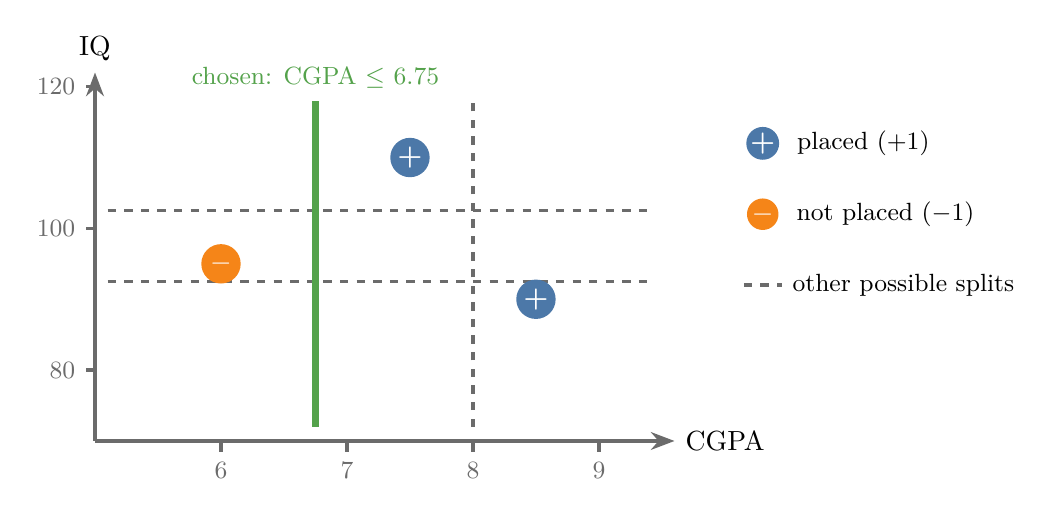
\begin{tikzpicture}[x=1.6cm, y=0.09cm]
  % axes: CGPA 5..9.5, IQ 70..120
  \draw[arrow] (5,70) -- (9.6,70) node[right] {CGPA};
  \draw[arrow] (5,70) -- (5,122) node[above] {IQ};
  \foreach \c in {6,7,8,9} \draw[cgrey] (\c,70) -- (\c,68.5) node[below, note] {\c};
  \foreach \q in {80,100,120} \draw[cgrey] (5,\q) -- (4.93,\q) node[left, note] {\q};
  % candidate splits (dashed) and the chosen one (solid)
  \draw[cgrey, dashed] (8,72) -- (8,118);
  \draw[cgrey, dashed] (5.1,92.5) -- (9.4,92.5);
  \draw[cgrey, dashed] (5.1,102.5) -- (9.4,102.5);
  \draw[cgreen, line width=2.2pt] (6.75,72) -- (6.75,118) node[above, font=\sffamily\small, text=cgreen] {chosen: CGPA $\le$ 6.75};
  % students
  \node[circle, fill=corange, minimum size=0.5cm, inner sep=0pt, text=white] at (6,95) {\textbf{$-$}};
  \node[circle, fill=cblue, minimum size=0.5cm, inner sep=0pt, text=white] at (7.5,110) {\textbf{+}};
  \node[circle, fill=cblue, minimum size=0.5cm, inner sep=0pt, text=white] at (8.5,90) {\textbf{+}};
  % legend
  \node[circle, fill=cblue, minimum size=0.4cm, inner sep=0pt, text=white] (l1) at (10.3,112) {\textbf{+}};
  \node[right=2pt of l1, font=\sffamily\small] {placed ($+1$)};
  \node[circle, fill=corange, minimum size=0.4cm, inner sep=0pt, text=white] (l2) at (10.3,102) {\textbf{$-$}};
  \node[right=2pt of l2, font=\sffamily\small] {not placed ($-1$)};
  \draw[cgrey, dashed] (10.15,92) -- (10.45,92) node[right, font=\sffamily\small, text=black] {other possible splits};
\end{tikzpicture}
\end{document}
